
The architecture of our system, called Text2KB, is presented on Figure \ref{fig:model}. 
The left part of the picture roughly corresponds to the architecture of existing information extraction approaches to knowledge base question answering.
In particular we based on system on the model developed in \cite{ACCU:2015}, which at the moment achieves the highest performance among the publicly available systems.
The right part of the figure shows examples of text resources that we use on different stages of the question answering process.
We will first describe the baseline system and then present extensions introduced in this work.

\begin{figure*}[t]
\centering
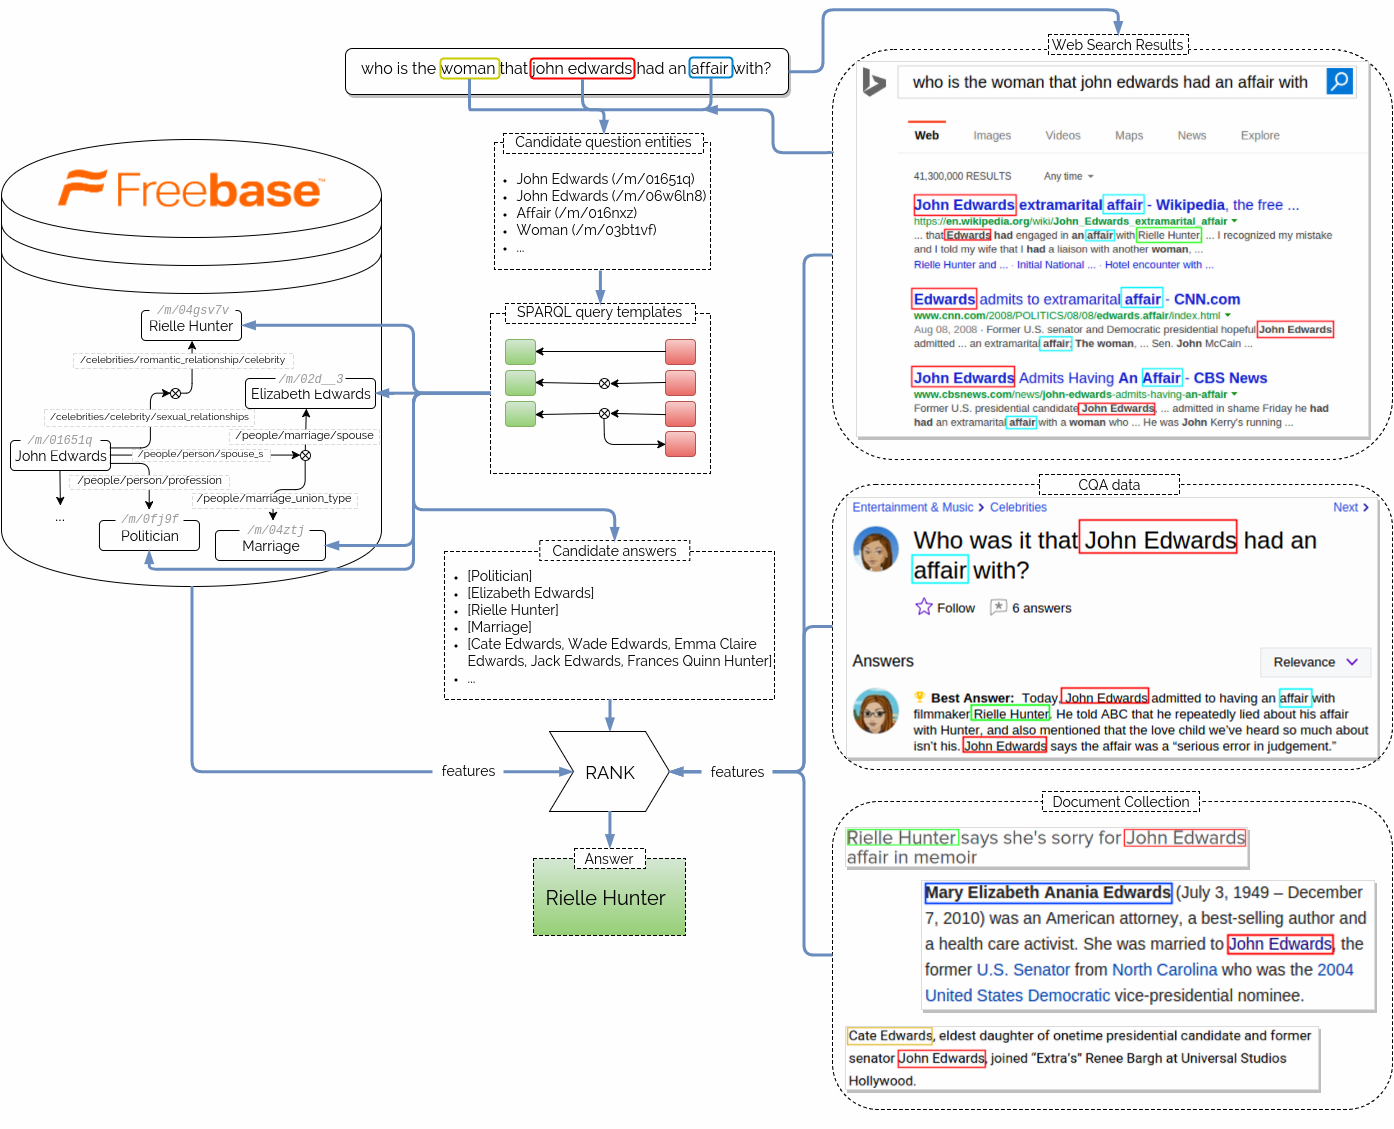
\includegraphics[width=\textwidth]{img/Text2KB_model}
\caption{The architecture of our Text2KB Question Answering system}
\label{fig:model}
\end{figure*}

\subsection{Unstructured text data for KBQA}

\subsubsection{Text data in KB}
We use entity descriptions to generate a set of features for candidate answers.
Description of entity in the knowledge base was found useful for question answering \cite{Sun:2015:ODQ:2736277.2741651}.
Therefore, we decided to use it as well.

Analogously, we can use entity Wikipedia profile pages.

\subsubsection{Web search results}
\label{section:method:web}

Our model issues the question as a query to a web search engine\footnote{https://datamarket.azure.com/dataset/bing/search} and extract top 10 results, \ie search snippets and corresponding documents.
Next, the system identifies KB entity mentions in both snippets and documents texts using the same method as used for question processing.
We use these data in two different ways: to extend the set of question entities and to generate features for candidate answer ranking.

\textbf{Question entity identification}.

In our system, Text2KB, we follow the following procedure to extend a set of identified KB entities identified from the question:
\begin{enumerate}
\item Detect entities mentioned in search result snippets and titles
\item An entity is added to the list of question entities if 
$$\max_{m_t \in M\backslash Stp, q_t \in Q\backslash Stp} dist(m_t, q_t) \geq 0.8$$
Here $M$ is a set of entity mention tokens, $Q$ - set of question tokens, dist() - text edit distance (we used Jaro-Winkler distance), and Stp is a set of stopwords.
\item For each question entity we count the number of mentions in search titles and snippets and use this information as a feature for answer candidate ranking.
\end{enumerate}

\textbf{Answer candidate features}.
Despite being useful for question entity identification, search results often contain the answer to the given question, \eg on Figure \ref{fig:web_search_entitylink} multiple snippets mention the date when Tutankhamun became the king.
Therefore, we use text of search results titles, snippets and documents to generate features for candidate answer ranking.
More specifically Text2KB computes the following:
\begin{enumerate}
\item Identify entities in search results titles, snippets and documents
\item Combine texts of all search result documents to form a single text (with entities identified)
\item Represent each snippet (which includes title), document and combined document as a two separate TF-IDF vectors: vector of term occurrences, vector of entity occurrences\footnote{We used Google n-grams corpus to approximate terms IDF and ClueWeb FACC entity annotations (http://lemurproject.org/clueweb09/FACC1/) to compute entity IDFs}
\item Each answer candidate is also represented as TF-IDF vectors of terms (from entity names) and entities
\item Compute cosine similarity between answer vectors and snippets, documents and combined document vectors and use maximum and average cosine similarities as features for candidate ranking.
\end{enumerate}

\subsubsection{Community Question Answering data}
\label{section:method:cqa}

Modern knowledge base question answering systems are typically trained from $<$question, answer entities$>$ pairs \cite{Berant:EMNLP13}, which are much easier to obtain than ground truth logical forms \cite{cai2013large}.
However, the sizes of available datasets are still rather small, \ie WebQuestions dataset of \cite{Berant:EMNLP13} contains only 5810 questions.
This is not enough for a system to be able to map a variety of natural language questions to tens of thousands of predicates in Freebase, each of which asked about in different ways.
Existing systems adapted additional data sources, such as question paraphrases \cite{berant2014semantic}, weakly labeled sentences from a large text collection \cite{yao2014information}.
However, often there exist a lexical gap between how information is asked about in a question and how it is expressed in a statement.
On the other hand, community question answering (CQA) websites contain millions of real users questions with answers, which makes them a very attractive source of data for training a QA system (\eg Figure \ref{fig:cqa_example}).

\begin{figure}
\centering
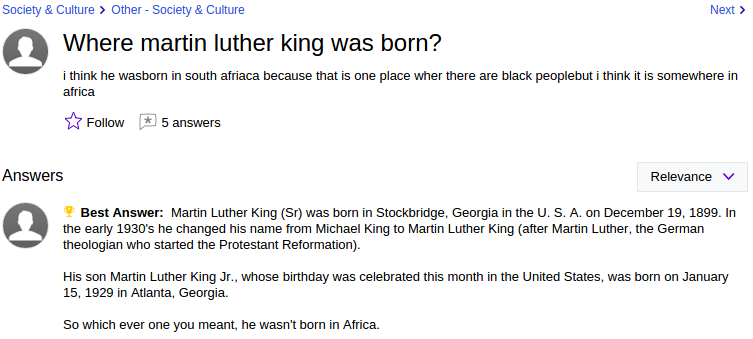
\includegraphics[width=0.5\textwidth]{img/cqa_example}
\caption{Example of a question and answer pair from Yahoo! Answers}
\label{fig:cqa_example}
\end{figure}

For our experiments we took 4,483,032 questions from Yahoo! Comprehensive Questions and Answers WebScope dataset\footnote{https://webscope.sandbox.yahoo.com/catalog.php?datatype=l}.
Texts of each question and answer pair were run through an entity linker, which detected mentions of Freebase entities.
Next, following the distant supervision heuristic, which were applied to CQA data for relation extraction \cite{savenkov-EtAl:2015:SRW}, we labeled each QnA pair with relations between entities mentioned in questions and answers.
To learn associations between predicates and questions that ask about these predicates, we compute pointwise mutual information scores (PMI) for pairs of question terms and predicates.
Examples of scores are given in Table \ref{table:cqa_npmi}.

\begin{table}
\caption{Examples of PMI scores for term-predicate pairs}
\label{table:cqa_npmi}
\begin{tabular}{| p{1.2cm} | p{5.0cm} | p{1.0cm} |}
\hline
Term & Predicate & PMI score\\
\hline
born & people.person.date\_of\_birth & 3.6706\\
 & people.person.date\_of\_death & 2.7364\\
 & people.person.place\_of\_birth & 1.6027\\
 & location.location.people\_born\_here & 1.6027\\
 & music.artist.origin & 1.2614\\
 & ... & ...\\
 & people.marriage.spouse & 0.6792\\
 & ... & ...\\
 & medicine.symptom.symptom\_of & -1.5312 \\
\hline
kill & people.deceased\_person.cause\_of\_death & 1.7066\\
& book.book.characters & 1.5500\\
& religion.religion.founding\_figures & 1.3008\\
& fictional\_universe.fictional\_character.species &  0.9195 \\
& ... & ... \\
& medicine.disease.causes & 0.3511 \\
& ... & ... \\
& people.person.profession & -0.1827\\
\hline
governor & government.government\_office\_or\_title.jurisdiction & 2.8042\\
& ... & ... \\
& location.country.administrative\_divisions & 1.2067\\
& people.person.profession & -0.4025 \\
\hline
currency & location.country.currency\_formerly\_used & 5.5505 \\
& location.country.currency\_used & 3.5433 \\
& ... & ...\\
& location.country.languages\_spoken & 0.9956\\
& ... & ...\\
& symbols.namesake.named\_after & -0.7669\\
\hline
school & education.school.school\_district & 4.1439 \\
& people.education.institution & 1.7083\\
& sports.school\_sports\_team.school & 1.6936 \\
\hline
continent & base.locations.countries.continent & 3.0850\\
& location.location.partially\_contains & 2.3436\\
& location.location.contains & 1.0527\\
\hline
illness & medicine.symptom.symptom\_of & 2.1167\\
& medicine.decease.causes & 1.6829\\
& medicine.disease.treatments & 1.5975\\
\hline
win & sports.sports\_team.championships & 4.1116\\
& sports.sports\_league.championship & 3.7924\\
\hline
\end{tabular}
\end{table}

These PMI statistics are used by our Text2KB system to generate features for each candidate answer, more specifically we compute minimum, maximum and average PMI score between candidate answer predicates and terms from the question.
Term statistics, however, is rather sparse, therefore for each predicate we also compute an embedding vector by taking a weighted (by PMI) average of embedding vectors of terms\footnote{we use pretrained word2vec term embeddings from https://code.google.com/p/word2vec/} with positive PMI value.
In testing time, for each question token we compute cosine similarity between its embedding vector and average predicate embedding vector and take minimum, maximum and average cosine similarity as features.

\subsubsection{Entity-linked collection of documents}
\label{section:method:clueweb}

Predicate in so called closed knowledge bases (such as dbPedia and Freebase) are represented with special identifiers, which while solving some problems complicates their mapping with natural language phrases.
Alternatively, open knowledge bases, such as ReVerb \cite{fader2011identifying}, extract information automatically from text sources and represent entities and predicate with natural language phrases.
This is useful for question answering \cite{Fader:2014:OQA:2623330.2623677}, which can now use the information on which terms and phrases are used in text collection to express relations between pairs of entities.
However, the extraction process isn't perfect and in particular suffers from low recall, which means that some information is lost.
To overcome this issue we propose to skip the extraction step and simply store information on text pieces used around entity pair mentions.
More specifically, we take ClueWeb12 corpus and use existing Freebase entity annotations\footnote{http://lemurproject.org/clueweb12/FACC1/} to collect statistics on terms that occur in the same sentence with an entity pair.
As a result, we have information on term counts for each pairs of entities.
In practice, to avoid splitting web documents into sentences we consider entity pairs that occur within 200 characters of each other and take terms between them and 100 characters to the left and right of mentions.
At the end we have the following data: $<e_1, e_2>: term_1: count, term_2: count$, ....
Table \ref{table:clueweb_entitypairs_langmodel} gives a couple of examples.

\begin{table}
\caption{Examples of entity pairs language model data}
\label{table:clueweb_entitypairs_langmodel}
\begin{tabular}{| p{1.25cm} | p{1.23cm} | p{4.5cm} |}
\hline
Entity 1 & Entity 2 & Term counts\\
\hline
John Edwards & Rielle Hunter & campaign, affair, mistress, child, former ...\\
\hline
John Edwards & Cate Edwards & daughter, former, senator, courthouse, left, greensboro, eldest ...\\
\hline
John Edwards & Elizabeth Edwards & wife, hunter, campaign, affair, cancer, rielle, husband ...\\
\hline
John Edwards & Frances Quinn Hunter & daughter, john, rielle, father, child, former, paternity...\\
\hline
\end{tabular}
\end{table}

Given an answer candidate we compute language model score for every answer candidate $$p(Q|e_1, e_2) = \prod_{t\in Q} p(t | e_1, e_2)$$ and use minimum, average and maximum score as features.
In addition, we compute weighted average embedding vector for a pair of entities by averaging the corresponding terms using their probabilities as weights and use minimum, average and maximum cosine similarity as features.

%\subsubsection{Wikipedia profile}
%It would be nice to have Wikipedia pages for entities and use something like SDM score or something else as feature.